First, the author used the reference count's timestamps as bins.
If there are multiple count of a group in one bin, the author calculated the average.
The reader can see in figure \ref{fig_comparison} and \ref{fig_comparison2} the group's count compared to the reference count.
To compare the group's counting algorithm performance better, the author calculated the absolute
difference to the reference count. Null values were replaced by zero for this calculation.\\
We can see that group 15 had the best performance and our counting algorithm (group 8) is on the
third place.

\begin{figure}
    \centering
    \begin{subfigure}[b]{0.45\textwidth}
        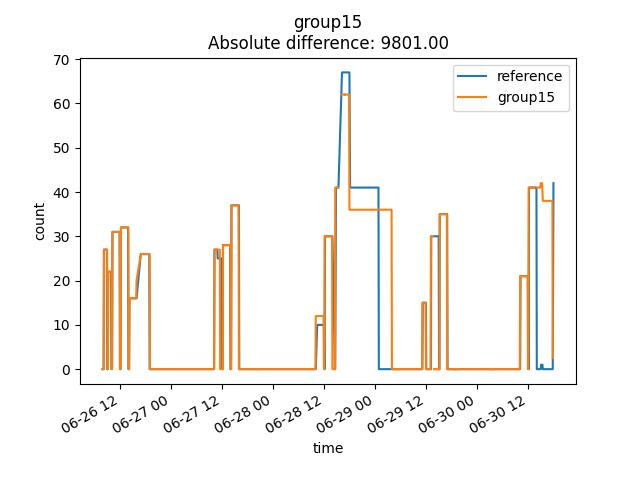
\includegraphics[width=\linewidth]{figures/ref-group15.jpeg}
        \caption{Place 1 of 9}
    \end{subfigure}
    \begin{subfigure}[b]{0.45\textwidth}
        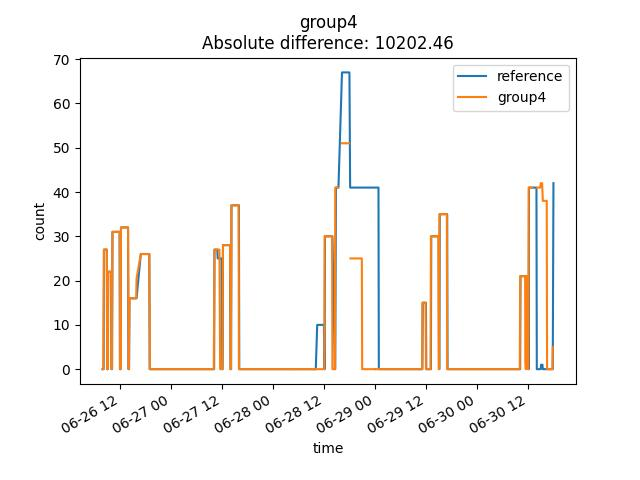
\includegraphics[width=\linewidth]{figures/ref-group4.jpeg}
        \caption{Place 2 of 9}
    \end{subfigure}

    \begin{subfigure}[b]{0.45\textwidth}
        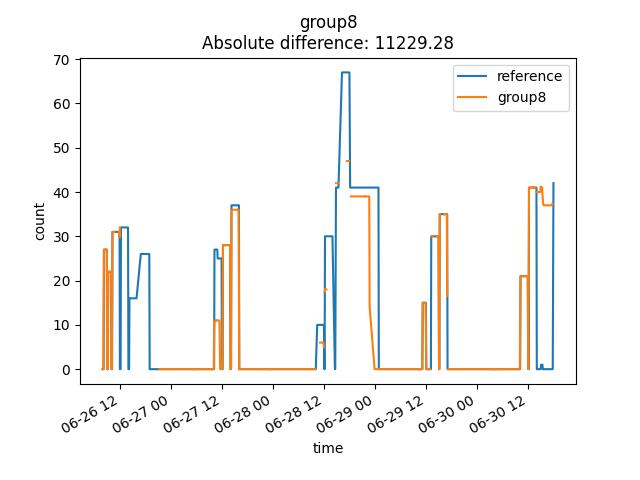
\includegraphics[width=\linewidth]{figures/ref-group8.jpeg}
        \caption{Place 3 of 9}
    \end{subfigure}
    \begin{subfigure}[b]{0.45\textwidth}
        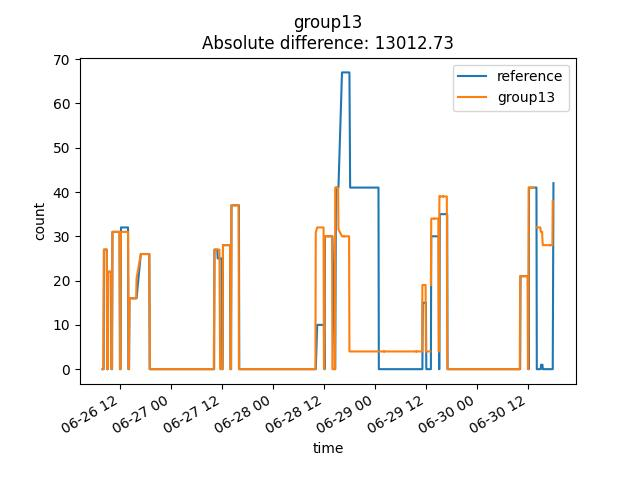
\includegraphics[width=\linewidth]{figures/ref-group13.jpeg}
        \caption{Place 4 of 9}
    \end{subfigure}

    \begin{subfigure}[b]{0.45\textwidth}
        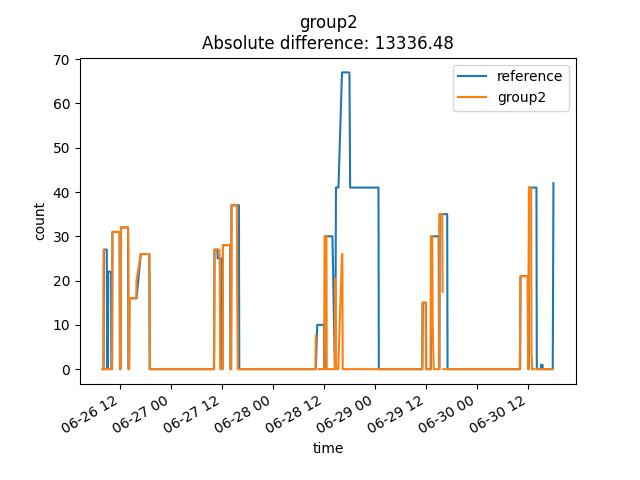
\includegraphics[width=\linewidth]{figures/ref-group2.jpeg}
        \caption{Place 5 of 9}
    \end{subfigure}
    \begin{subfigure}[b]{0.45\textwidth}
        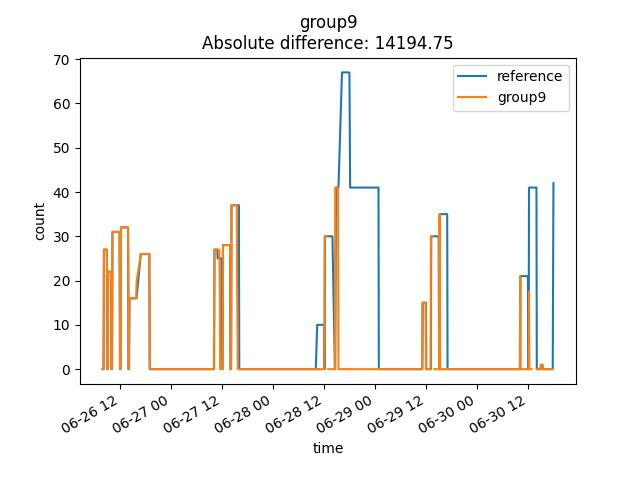
\includegraphics[width=\linewidth]{figures/ref-group9.jpeg}
        \caption{Place 6 of 9}
    \end{subfigure}

    \caption{Group comparison. The absolute difference (in seconds) is the absolute difference to the reference count.
        The pictures are ordered descending by their counting algorithm performance.}
    \label{fig_comparison}
\end{figure}

\begin{figure}
    \begin{subfigure}[b]{0.45\textwidth}
        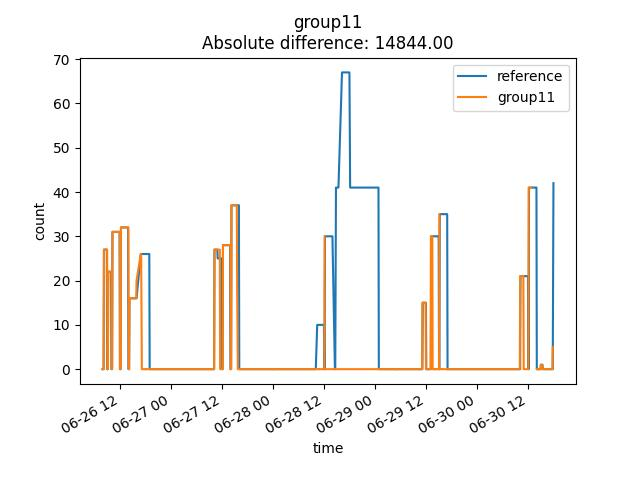
\includegraphics[width=\linewidth]{figures/ref-group11.jpeg}
        \caption{Place 7 of 9}
    \end{subfigure}
    \begin{subfigure}[b]{0.45\textwidth}
        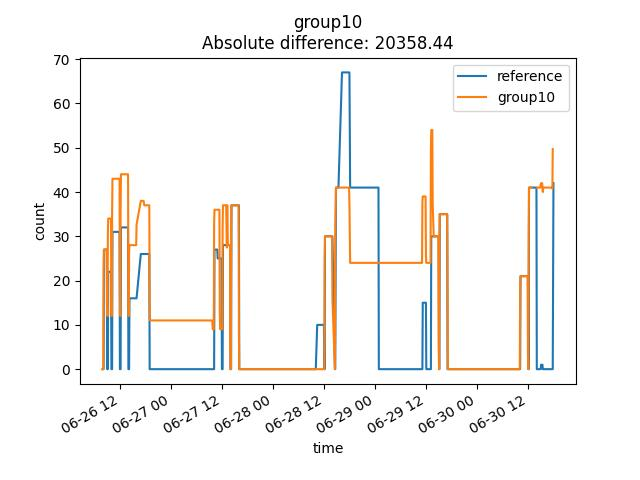
\includegraphics[width=\linewidth]{figures/ref-group10.jpeg}
        \caption{Place 8 of 9}
    \end{subfigure}

    \begin{subfigure}[b]{0.45\textwidth}
        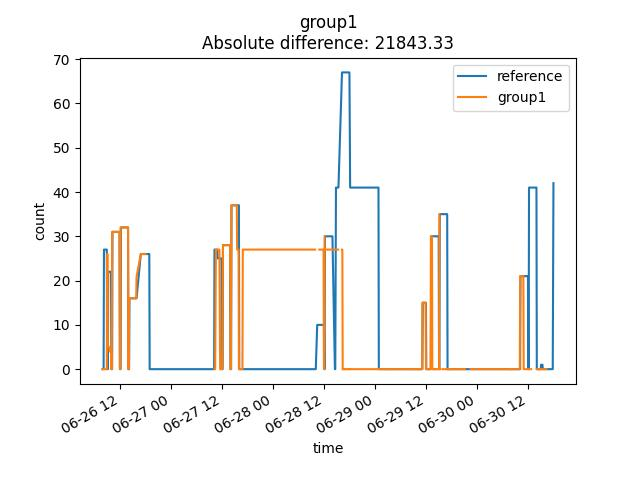
\includegraphics[width=\linewidth]{figures/ref-group1.jpeg}
        \caption{Place 9 of 9}
    \end{subfigure}
    \caption{Group comparison. The absolute difference (in seconds) is the absolute difference to the reference count.
        The pictures are ordered descending by their counting algorithm performance.}
    \label{fig_comparison2}
\end{figure}